\documentclass[12pt,a4paper]{article}
\usepackage{listings}
\usepackage{geometry}
\usepackage{setspace}
\usepackage{fancyhdr}
\usepackage{graphicx}
\usepackage{xcolor}
\usepackage{polyglossia}
\usepackage{hyperref}

\setdefaultlanguage{greek}
\setotherlanguage{english}
\setmainfont{Times New Roman}
\newfontfamily\greekfont{Times New Roman}
\newfontfamily\englishfont{Times New Roman}

\setlength{\headheight}{15pt}

\geometry{margin=2.5cm}
\doublespacing
\pagestyle{fancy}
\fancyhf{}
\fancyhead[R]{\thepage}
\fancyhead[L]{Έξυπνο Συμβόλαιο Διαχείρισης Στοιχείων Κατοικιδίων}


\begin{document}

% Define colors
\definecolor{solidityKeyword}{rgb}{0.0,0.2,0.6}   % dark blue
\definecolor{solidityType}{rgb}{0.6,0.1,0.6}      % purple
\definecolor{solidityComment}{rgb}{0.25,0.5,0.35} % green
\definecolor{solidityString}{rgb}{0.6,0.2,0.2}    % reddish

% Fix for monospace fonts in Greek/English
\newfontfamily\greekfonttt{Courier New}
\newfontfamily\englishfonttt{Courier New}

% Define Solidity language
\lstdefinelanguage{Solidity}{
  keywords={
    contract,library,interface,struct,event,enum,function,modifier,
    constructor,fallback,receive,returns,import,pragma,storage,memory,calldata,
    if,else,for,while,do,break,continue,return,emit,revert,require,assert,new,
    mapping,this,super,delete,using,as,assembly
  },
  keywordstyle=\color{solidityKeyword}\bfseries,
  ndkeywords={address,bool,string,bytes,int,uint,int8,uint8,int16,uint16,
    int32,uint32,int64,uint64,int128,uint128,int256,uint256,byte,ufixed,fixed},
  ndkeywordstyle=\color{solidityType}\bfseries,
  sensitive=true,
  comment=[l]{//},
  commentstyle=\color{solidityComment}\ttfamily,
  morecomment=[s]{/*}{*/},
  stringstyle=\color{solidityString}\ttfamily,
  morestring=[b]",
  morestring=[b]'
}

% Default style
\lstset{
  language=Solidity,
  basicstyle=\ttfamily\footnotesize,
  numbers=left,
  numberstyle=\tiny\color{gray},
  stepnumber=1,
  numbersep=5pt,
  showstringspaces=false,
  tabsize=2,
  breaklines=true,
  frame=single,
  rulecolor=\color{black!30},
  captionpos=b
}


\begin{titlepage}
    \centering
    \vspace*{2cm}
    
    {\huge\textbf{Έξυπνο Συμβόλαιο Διαχείρισης Στοιχείων Κατοικιδίων}}\\
    \vspace{2cm}
    {\large Προγραμματιστική Εργασία Solidity (2025)}
    \vspace{3cm}
    
    {\large\ \textbf{Μάθημα:} Τεχνολογίες Blockchain \& Εφαρμογές}\\
    {\large\ \textbf{Καθηγήτρια:} Δρ. Αριστέα Κοντογιάννη}\\
    \vspace{2cm}
    
    {\large Γιώργος Νικολαΐδης (π21115)}\\
\end{titlepage}

\tableofcontents
\newpage

\section{Εισαγωγή}
Η παρούσα εργασία εμπεριέχει ένα αρχείο κώδικο Solidity που ορίζεται ένα έξυπνο συμβόλαιο ονόματι "\textbf{Pets}". Το συμβόλαιο καθορίζει πέντε μεθόδους (functions), η κάθε μέθοδος υλοποιεί μια λειτουργία που ορίζει η εκφώνηση. 

Στις δύο ενότητες που ακολουθούν, θα αναλυθεί περαιτέρω ο κώδικας και θα φανεί σε πράξη η λειτουργία του έξυπνου συμβόλαιου.

\newpage

\section{Ανάλυση Κώδικα}

\subsection{Ο Κώδικας}
\lstinputlisting[language=Solidity]{../contracts/Pets.sol}

\subsection{Τα Μέρη του Συμβολαίου}
Το συμβόλαιο εσωτερικά είναι χωρισμένο σε διάφορα μέρη.

\subsubsection{Ορισμός Δομών Δεδομένων}
Στο συμβόλαιο γίνεται η χρήση ειδικών δομών δεδομένων (struct) για να επιτευχθεί η ορθή και ξεκάθαρη μοντελοποίηση του προβλήματος.

\begin{itemize}
    \item \textbf{Pet}: Μοντελοποιεί τις ιδιότητες ενός κατοικιδίου, όπως ορίζεται στην εκφώνηση της εργασίας. Δεν έχει πεδίο για τον μοναδικό κωδικό chip (Chip ID), η ταυτοποίηση με τον κωδικό γίνεται σε σημείο που θα δούμε αμέσως μέτα. Αξίζει να σημειωθεί η παρουσία των ιδιοτήτων \textbf{createdAt} και \textbf{modifiedAt}, η οποίες υπάρχουν για λόγους auditing - να μπορεί οποιοσδήποτε να δεί πότε δημιουργήθηκε/ενημερώθηκε ένα κατοικίδιο.
    
    \item \textbf{PetStatus}: Παρέχει πληροφορίες για την κατάσταση του κατοικιδίου - αν είναι ενεργό στο σύστημα και μια αιτιόλογηση για αν δεν είναι.
\end{itemize}

\subsubsection{Μεταβλητές Κατάστασης (State Variables)}
Για την αποθήκη των δεδομένων των κατοικιδίων χρησιμοποιούνται δύο state variables:

\begin{itemize}
    \item \textbf{pets}: Είναι ένας πίνακας κατακερματισμού (hash table) με κλειδί το μοναδικό κωδικό chip (Chip ID) και τιμή ένα κατοικίδιο. Αποτελεί τη μεταβλητή στην οποιά αποθηκεύονται όλα τα δεδομένα των κατοικιδίων που εισάγωγονται/ενημερώνονται.\
    \item \textbf{existingPets}: Βοηθητικός πίνακας κατακερματισμού για να αναγνωρίζει το συμβόλαιο αν κάποιο κατοικίδιο είναι καταχωριμένο στο δεδομένα του. Η ανάγκη για αυτή τη μεταβλητή υπάρχει λόγω της ειδικής υλοποιήσης του πίνακα κατακερματισμού από τη Solidity. Στο  \href{https://docs.soliditylang.org/en/v0.8.30/types.html#mapping-types}{documentation της γλώσσας}, αναγράφεται ότι: \begin{quote}
        You can think of mappings as hash tables, which are virtually initialised such that every possible key exists and is mapped to a value whose byte-representation is all zeros, a type’s default value... Because of this, mappings do not have a length or a concept of a key or value being set, and therefore cannot be erased without extra information regarding the assigned keys
    \end{quote}
\end{itemize}

\subsubsection{Function Modifiers}
Οι function modifiers μπορούν να χαρακτηριστούν ως "Decorators" (από το Decorator design pattern), επείδη επεκτήνουν την λειτουργία των μεθόδων που αναθέτονται χώρις να είναι μέρος της υλοποιήσης τους.

Στην περίπτωση της παρούσας εργασίας, χρησιμοποιούνται για την επικύρωση των εισόδων που δέχονται οι μέθοδοι. Με σκοπό την πρόωρη επιστροφή σε περίπτωση που υπάρχει σφάλμα στις εισόδους. Ορίζουμε δύο modifiers:
\begin{itemize}
    \item \textbf{petExists}: Ελέγχει αν ο μοναδικός κωδικός chip είναι καταχωριμένος στο σύστημα. Αν δεν υπάρχει, επιστρέφει πρόωρα ένα μήνυμα επικύρωσης στον caller.
    \item \textbf{petDoesNotExist}: Ελέγχει αν ο μοναδικός κωδικός chip είναι καταχωριμένος στο σύστημα. Αν υπάρχει, επιστρέφει πρόωρα ένα μήνυμα επικύρωσης στον caller.
\end{itemize}

\subsubsection{Λειτουργίες (Functions)}
Εδω βρίσκονται οι λειτουργίες του συμβολαίου οι οποίες είναι \textbf{public} για να μπορούν να τις καλούν χρήστες ή άλλα συμβόλαια. Οι λειτουργίες, αναλυτικά, είναι:

\begin{itemize}
    \item \textbf{add}: Υλοποιεί τη λειτουργία "\textbf{Καταχώρηση νέου κατοικίδιου}" απο την εκφώνηση. Δέχεται ως εισόδους κωδικό chip, όνομα, είδος και ηλικία κατοικιδίου.
    
    Προτού γίνει η καταχώρηση, κάθε είσοδος ελέγχεται ως προς την ορθότητα της. Εαν τουλάχιστον μια είσοδος δεν είναι έγκυρη, το συμβόλαιο δεν προχωράει στην καταχώρηση του κατοικιδίου.

    Αν όλες οι εισόδοι είναι έγκυρες, τότε αρχικοποιείται ένα καινούργιο κατοικίδιο \textbf{Pet} και καταχωρείται απευθίας στον πίνακα \textbf{pets}. Σημειώνεται επίσης στον πίνακα \textbf{existingPets} ότι το κατοικίδιο με κωδικό \textbf{chipId} υπάρχει.

    \item \textbf{updateName}: Υλοποιεί τη λειτουργία "\textbf{Ενημέρωση στοιχείων κατοικίδιου}" της εκφώνησης. Δέχεται ως είσοδο το κωδικό chip του κατοικίδιο που θα αλλάξει το όνομα και το καινούργιο όνομα.
    
    Πριν αλλάξει το όνομα, επικυρώνεται ο κωδικός chip ότι υπάρχει και το καινούργιο όνομα οτι δεν είναι κενό.

    Αν όλες οι εισόδοι είναι έγκυρες, τότε η μέθοδος παίρνει μια αναφορά του αποθηκευμένου κατοικιδίου με κωδικό = \textbf{chipId}, και θέτει στο στιγμιότυπο το καινούργιο όνομα. 
    
    Η χρήση της λέξης \textbf{storage} στην εντολή αποθήκευσης είναι άκρως σημαντική, γιατι λέμε στην EVM (Ethereum Virtual Machine) ότι χρειαζόμαστε ένα pointer/reference του στιγμιότυπου του κατοικιδίου. Αν χρησιμοποιούσαμε \textbf{memory} ή \textbf{calldata} τότε θα λαμβάναμε ένα αντίγραφο του στιγμιότυπου, που θα σήμαινε ότι όποια αλλαγή κάναμε θα γινόταν πάνω στο αντίγραφο και όχι στο αρχικό στιγμιότυπο. 

    \item \textbf{incrementAge}: Υλοποιεί τη λειτουργία "\textbf{Εξέλιξη ηλικίας κατοικίδιου}" της εκφώνησης. Δέχεται ως είσοδο το κωδικό chip του κατοικιδίου που θέλουμε η ηλικία να αυξηθεί.
    
    Αν ο κωδικός chip υπάρχει και η ηλικία του κατοικιδίου δεν ξεπερνάει ένα όριο, τότε η μέθοδος αυξάνει την ηλικία κατα 1.

    \item \textbf{softDelete}: Υλοποιεί τη λειτουργία "\textbf{Δήλωση απομάκρυνσης κατοικίδιου}" της εκφώνησης. Δέχεται είσοδο κωδικό chip και μια αιτιόλογηση.
    
    Αρχικά επικυρώνεται η υπάρξη του κατοικιδίου και ύστερα τροποποιείται το κατοικίδιο να φαίνεται "ανενεργό" στο συμβόλαιο.

    \item \textbf{get}: Υλοποιεί τη λειτουργία "\textbf{Ανάκτηση στοιχείων κατοικίδιου}" της εκφώνησης. Δέχεται ως είσοδο ένα κωδικό chip.
    
    Στον ορισμό της μεθόδου δηλώνεται ότι είναι \textbf{view} και ότι επιστρέφει ένα \textbf{Pet}. Το \textbf{view} διαβεβαιώνει την EVM ότι η συγκεκριμένη μεθόδος ΔΕΝ τροποποιεί δεδομένα και απλώς επιστρέφει, λέγεται και \textbf{pure function}.
    
    Στην υλοποίηση της μεθόδου, γίνεται έλεγχος ότι το κατοικίδιο υπάρχει και αν υπάρχει επίστρεφεται όπως είναι.
\end{itemize}

\section{Στιγμιότυπα Οθόνης}

\begin{figure}[ht]
    \centering
    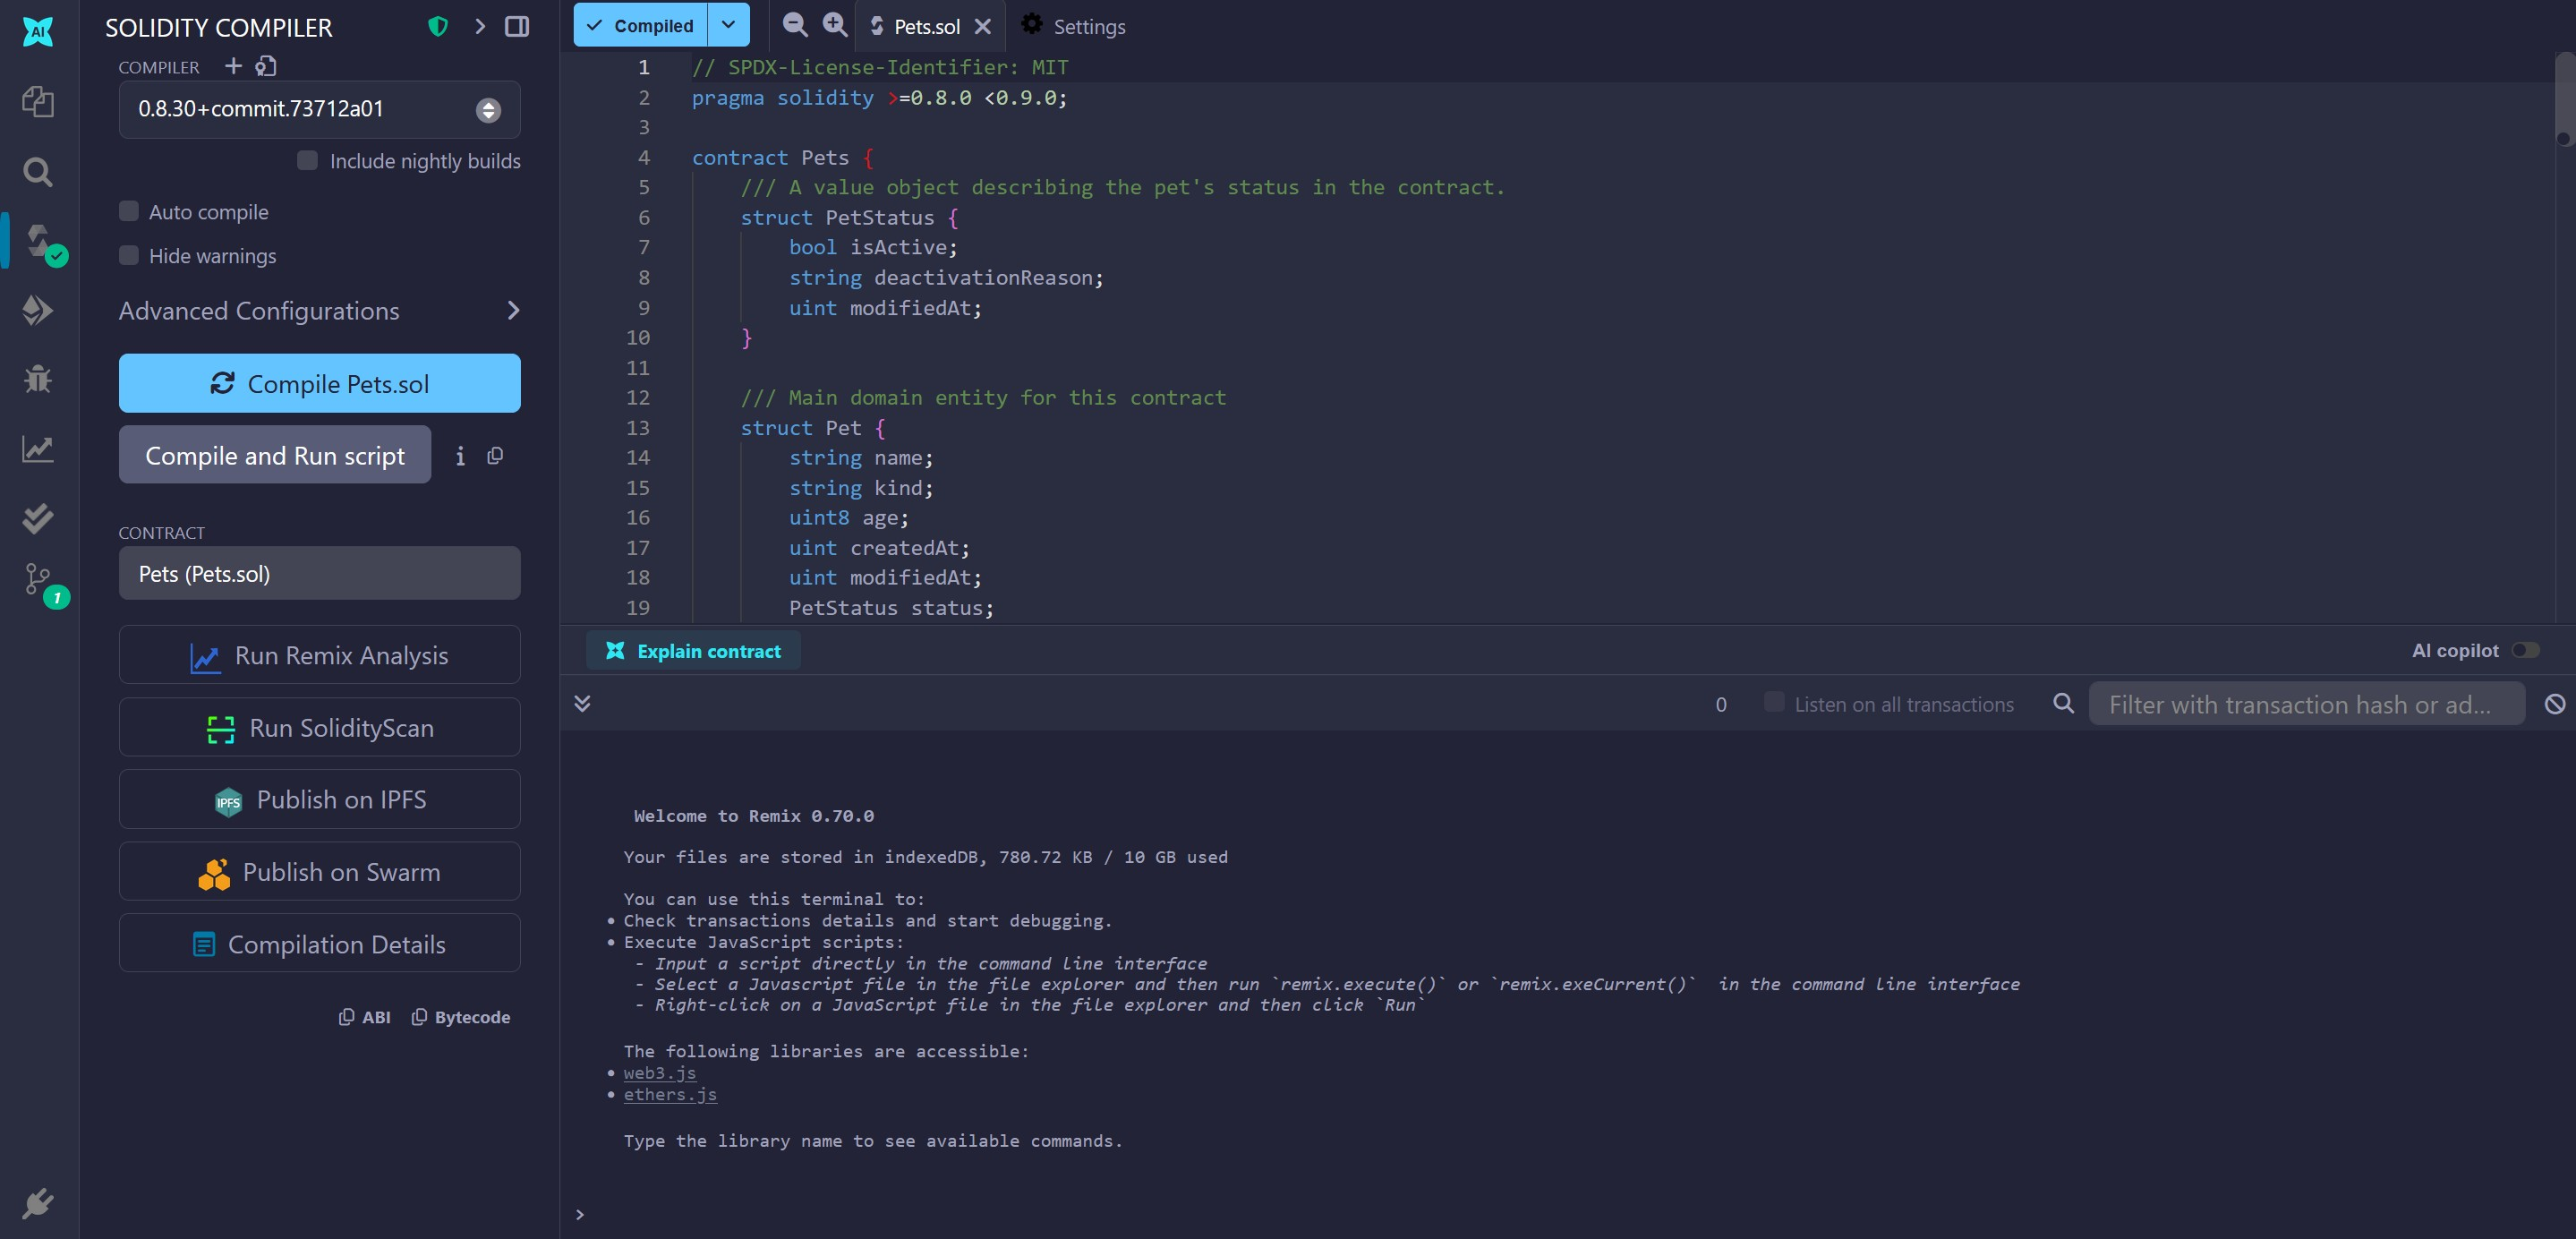
\includegraphics[width=\textwidth]{img/compile.jpg}
    \caption{Επιτυχής μεταγλώττιση του συμβολαίου}
\end{figure}

\begin{figure}[ht]
    \centering
    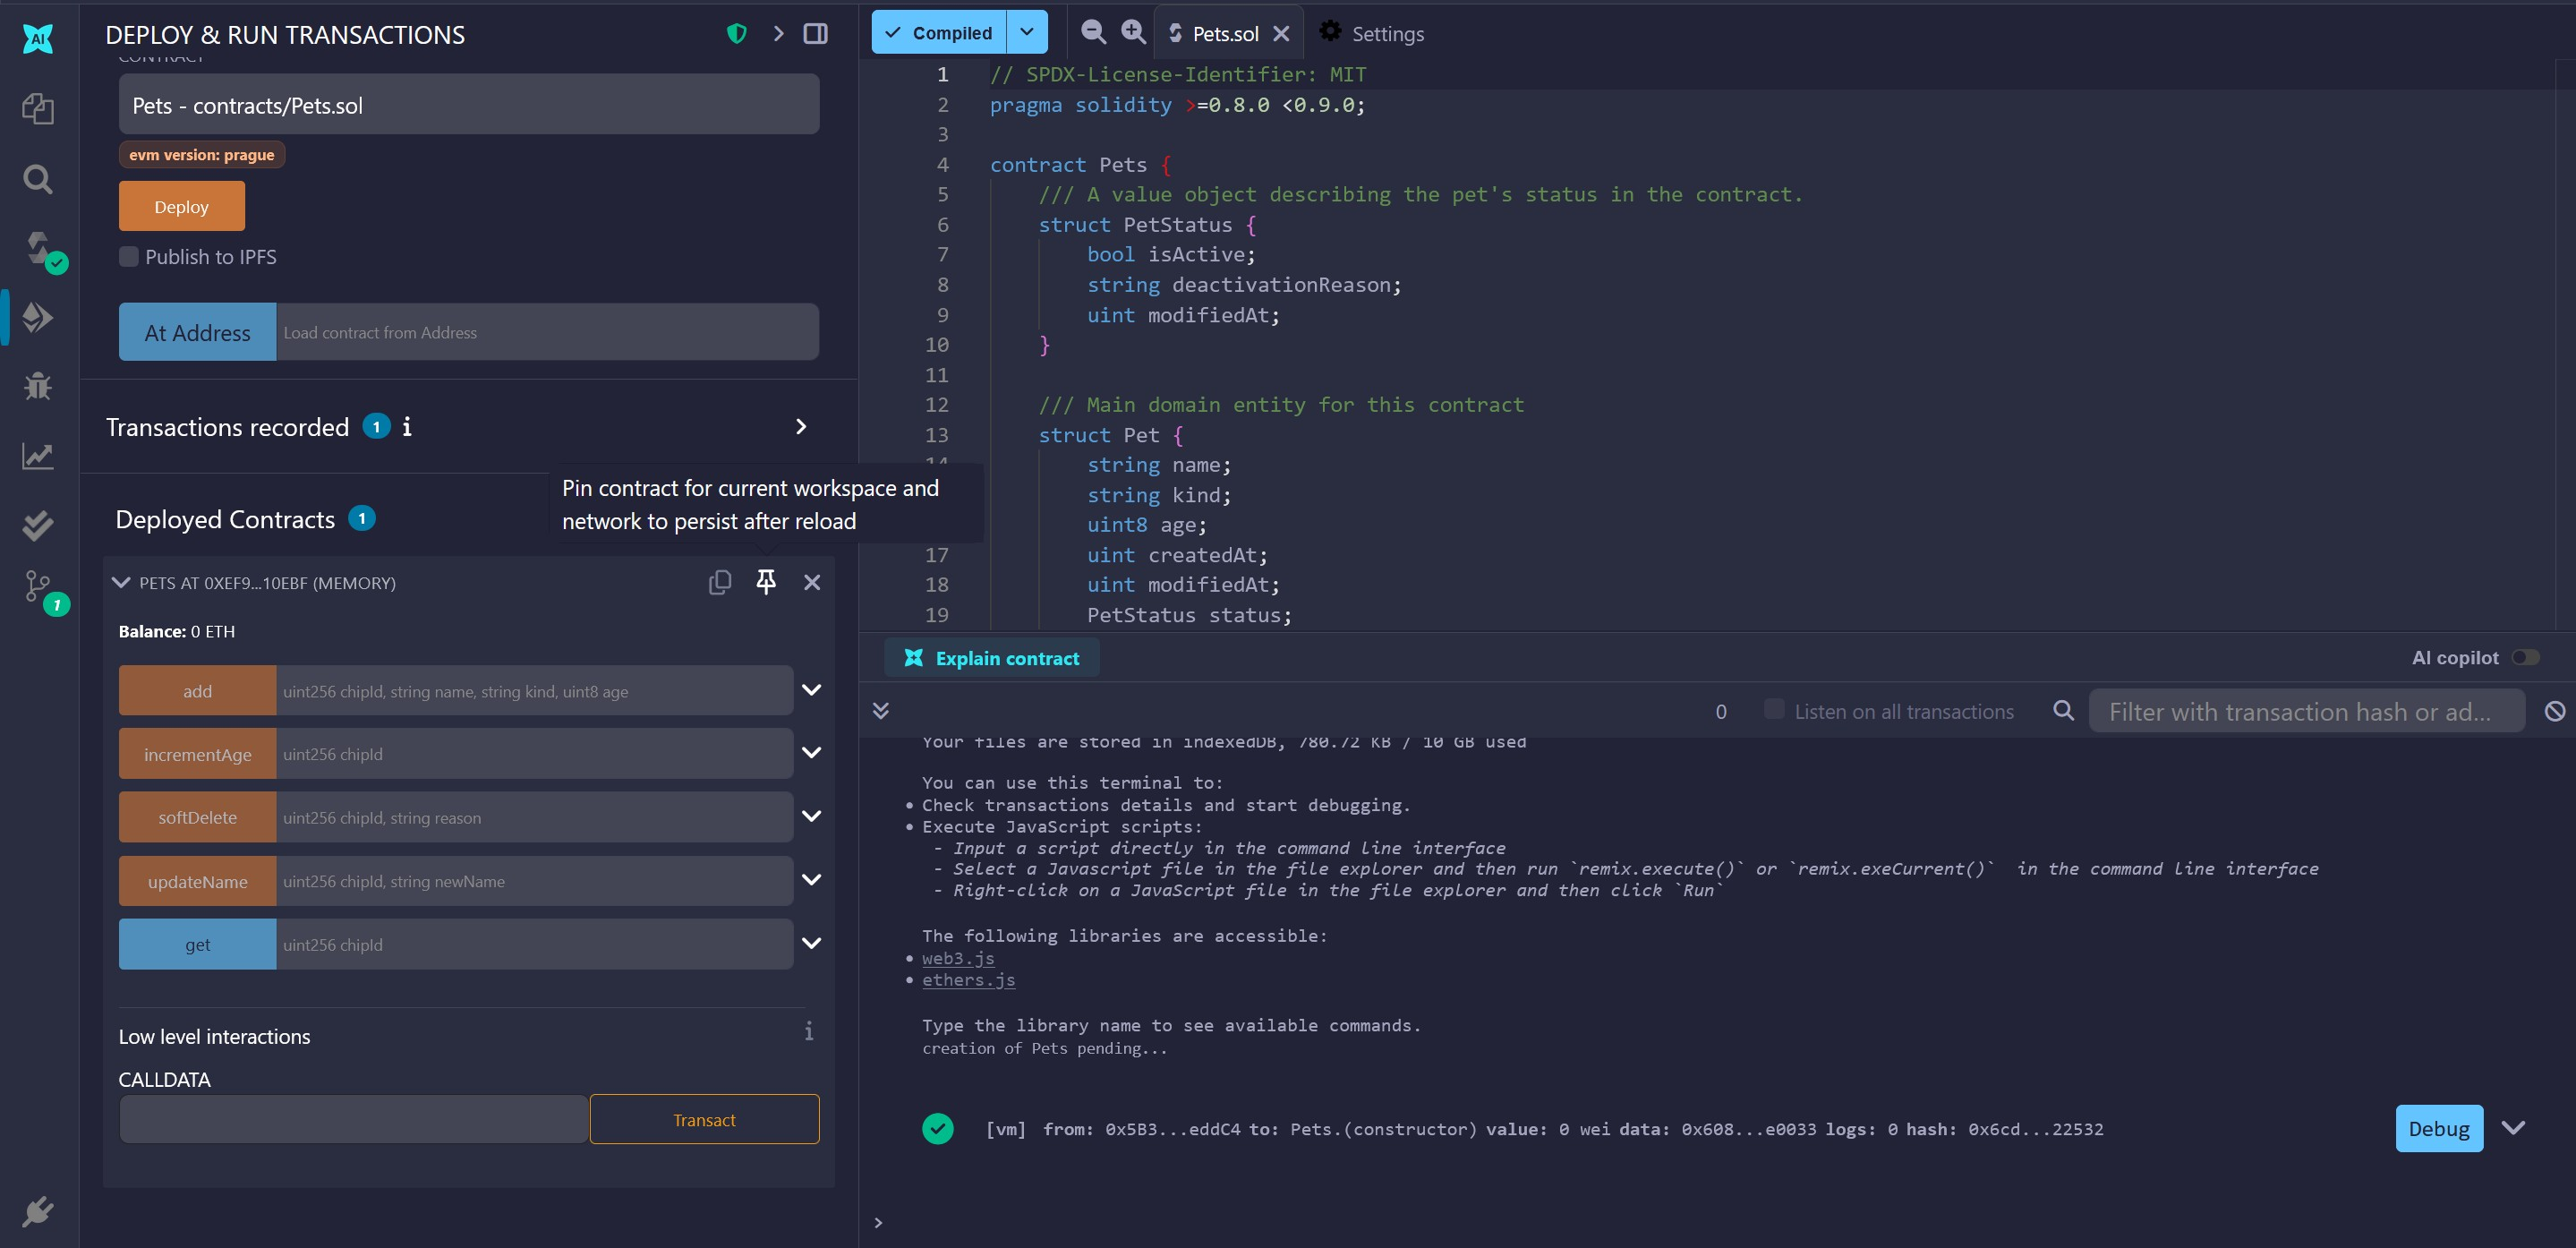
\includegraphics[width=\textwidth]{img/deploy.jpg}
    \caption{Επιτυχής δημιουργία (deployment) του συμβολαίου}
\end{figure}

\begin{figure}[ht]
    \centering
    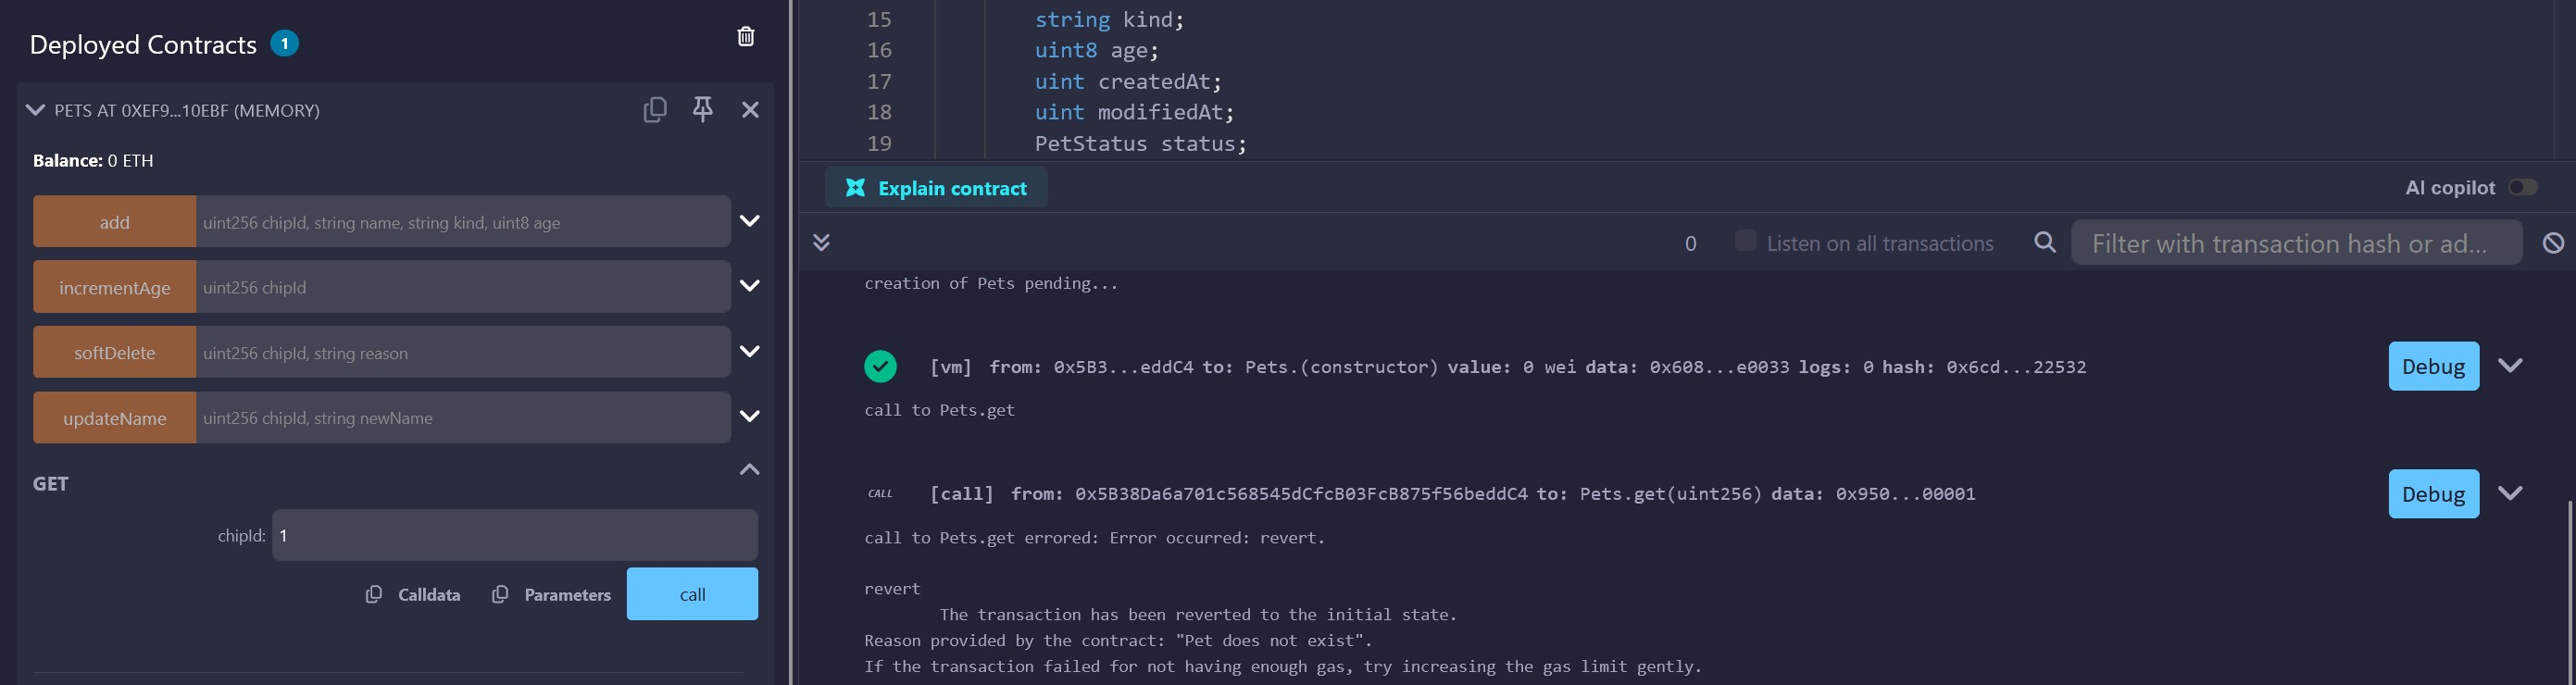
\includegraphics[width=\textwidth]{img/get_fail.jpg}
    \caption{Ανάκτηση κατοικιδίου όταν δεν υπάρχει ο δοσμένος κωδικός chip}
\end{figure}

\begin{figure}[ht]
    \centering
    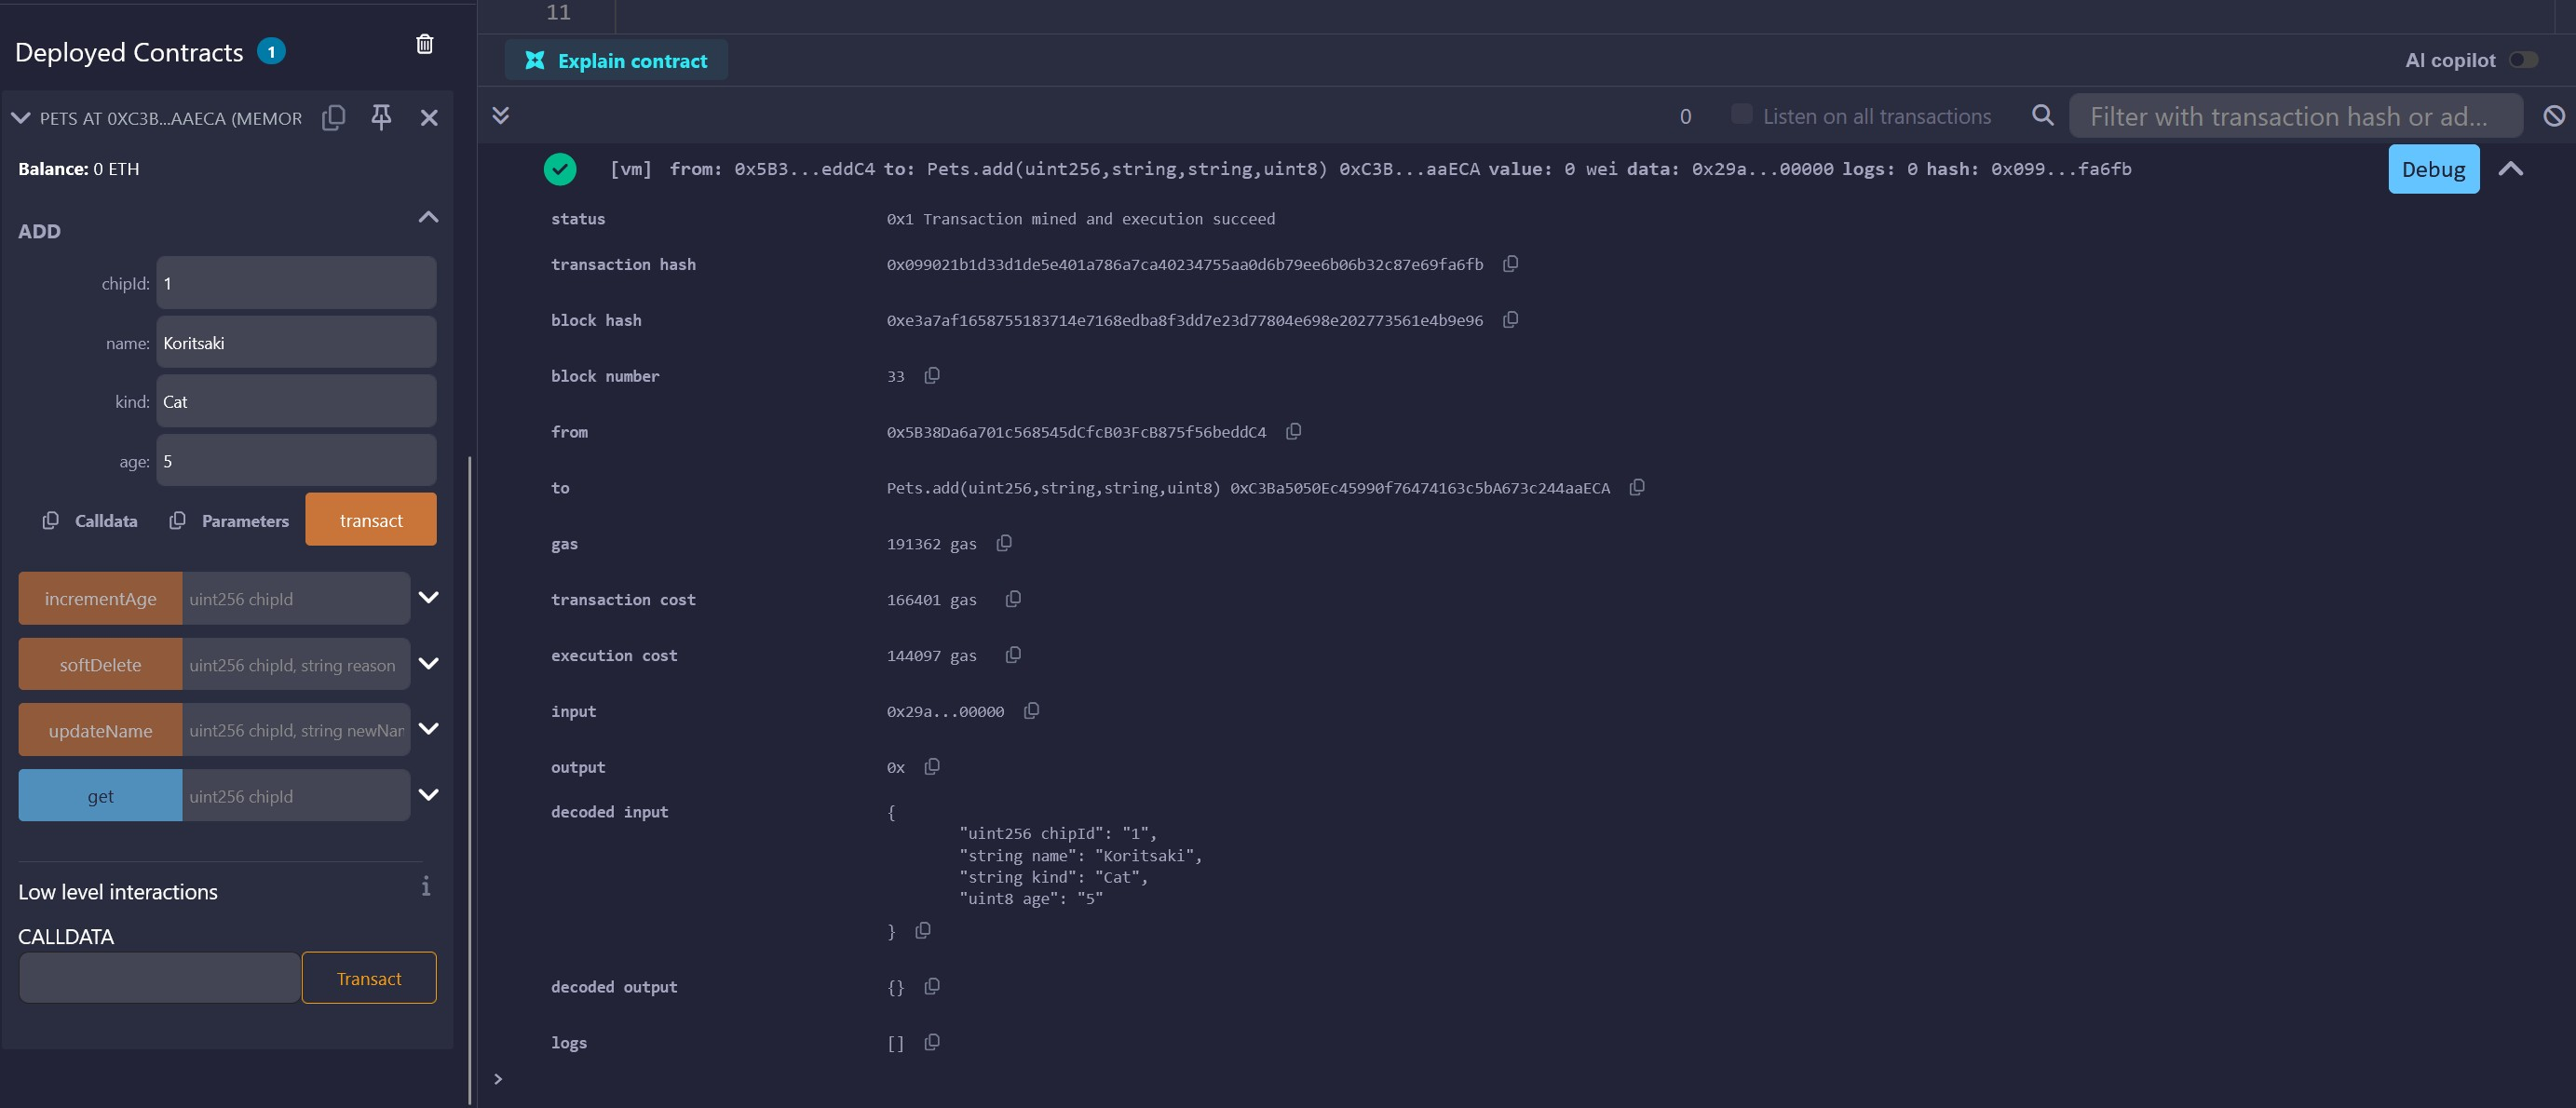
\includegraphics[width=\textwidth]{img/add_success.jpg}
    \caption{Καταχώρηση κατοικιδίου με έγκυρο κωδικό chip και στοιχεία}
\end{figure}

\begin{figure}[ht]
    \centering
    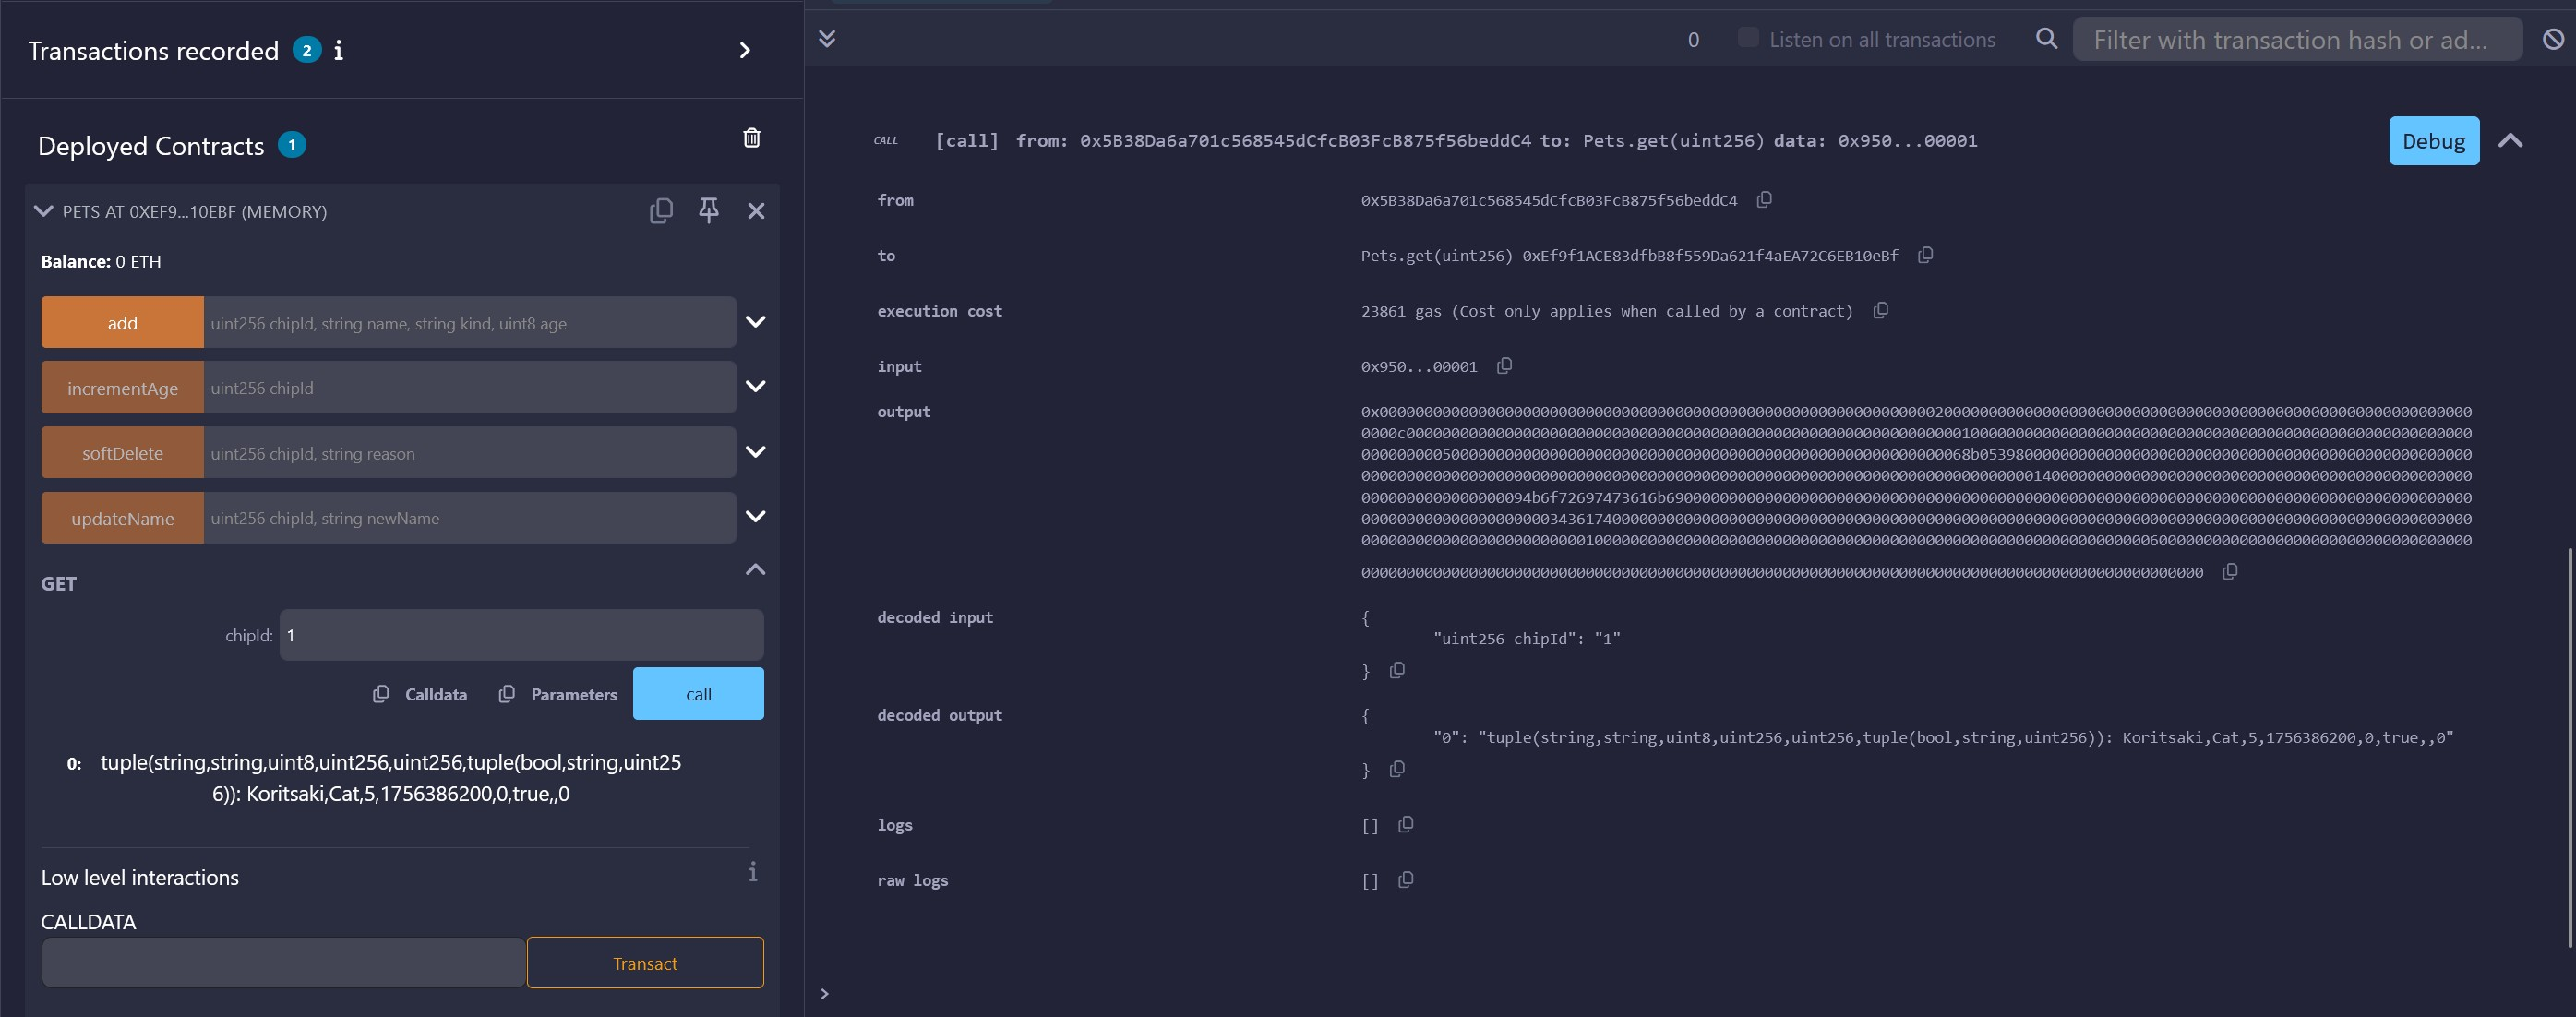
\includegraphics[width=\textwidth]{img/get_success.jpg}
    \caption{Ανάκτηση κατοικιδίου όταν υπάρχει ο κωδικός chip}
\end{figure}

\end{document}